\documentclass[11pt,a4paper,onecolumn]{article}
\usepackage[margin=27mm]{geometry}
\usepackage[T1]{fontenc}
\usepackage{lmodern,microtype,ragged2e,setspace,graphicx,booktabs,tabularx,array,amsmath,amssymb,caption,subcaption,float,xcolor,hyperref}
\usepackage[numbers,sort&compress]{natbib}
\hypersetup{colorlinks=true,citecolor=black,linkcolor=black,urlcolor=blue}
\setstretch{1.1}\setlength{\parindent}{0pt}\setlength{\parskip}{5pt}
\AtBeginDocument{\RaggedRight}
\captionsetup{font=small,justification=raggedright,singlelinecheck=false}
\newcolumntype{Y}{>{\RaggedRight\arraybackslash}X}
\title{Evidence-Aware Correlation and Constrained Reconstruction of Cybersecurity Incidents under Incomplete Telemetry}
\author{Hunain Shahid \and Hammad Ullah Khan}
\date{}
\begin{document}\maketitle
\begin{abstract}\RaggedRight
Security alert grouping is risky when multiple apparent corroborating claims descend from one observation, arrive after the decision time, or disagree about event identity. We examine a constrained correlation, verification, and prioritization pipeline that forms initial alert fragments, accepts cross-fragment relationships only under explicit provenance and consistency checks, and ranks the resulting groups. A narrowly scoped endpoint fallback substitutes original endpoint process context for a missing process claim only when timely, independent authentication and network observations support the same relationship. We compare this frozen candidate against a matched frozen baseline on an untouched, controlled synthetic holdout of 15 queues and 5,018 eligible alerts. Incident Recall@20 rose from 250/300 (83.33\%) to 260/300 (86.67\%); group recoverability rose from 263/300 (87.67\%) to 281/300 (93.67\%); and P@10 rose from 107/150 (71.33\%) to 113/150 (75.33\%). Both pipelines had zero false grouped pairs and zero mixed groups under simulator truth. The candidate had missed its development gate by one incident, and the subsequent decision to evaluate it unchanged on fresh holdout data was documented before the test. Later ranking studies on separate development cohorts did not establish a reliable improvement. An audit of public real-world evidence found missing provenance and point-in-time fields; consequently no external performance evaluation was conducted. The findings characterize a synthetic evidence model, not operational SOC validity.
\end{abstract}

\noindent\textbf{Keywords:} security operations; alert correlation; incident reconstruction; evidence provenance; temporal availability; incident prioritization
\section{Introduction}
Security operations centers must turn many detector outputs into a smaller number of reviewable incidents. Aggregation can reduce an analyst's workload, but a plausible relationship is not necessarily a trustworthy relationship: a copied claim may look like an independent witness, an event timestamp may precede the time its evidence became available, and a shared host or account may join unrelated activity. Research on domain-independent aggregation, multi-stage reconstruction, and triage addresses different parts of this problem \citep{landauer2022,wang2024,grain2025,sadlek2025}. The safety of a reconstructed incident depends on the evidence that justifies each cross-fragment union.

We study a specific decision problem: at a fixed cutoff, partition the alerts that have become visible into incident candidates, while refusing a cross-fragment link when its attestation is unavailable, dependent, inconsistent, or contradicted. The resulting groups are ranked for analyst review. Correlation proposes relationships; verification controls which extra unions can occur; ranking cannot repair a missing group. Prior work often emphasizes alert reduction, attack prediction, graph reconstruction, or prioritization, and these objectives and their labels are not interchangeable \citep{malach2025,grain2025,chuah2025}.

Our questions are: (RQ1) how does the implemented provenance and point-in-time verifier constrain cross-fragment reconstruction under incomplete evidence; (RQ2) does an endpoint-based fallback improve recoverability and retrieval on a matched, untouched synthetic holdout without observed unsafe unions; and (RQ3) what evidence limits further ranking gains and a valid external test? The contributions are an implementable account of the verifier and constrained fallback, a paired synthetic holdout comparison with group-safety measures, and a documented external data-readiness audit. We make no claim of superiority over published systems on incompatible datasets. Sections 2--5 establish the design; Sections 6--8 specify and report its evaluation; the remaining sections discuss interpretation and external validity.

\section{Background and related work}
\subsection{Aggregation, reconstruction, and prioritization}
Landauer et al. learn domain-independent patterns for aggregating semi-structured alerts \citep{landauer2022}. Wang et al. combine similarity-based aggregation with a Transformer for multi-stage attack prediction \citep{wang2024}. GRAIN discovers potential causal relationships and uses graph learning and reinforcement learning for attack-scenario reconstruction \citep{grain2025}. These systems answer different questions from whether a particular candidate edge has three original, point-in-time, independently rooted observations. Their published evaluation protocols and datasets do not permit a fair numeric comparison with ours.

Sadlek et al. use kill-chain attack graphs to prioritize incidents by severity \citep{sadlek2025}; CyberShapley explains and prioritizes anomaly-detection components \citep{malach2025}. Neither task is identical to reconstructing a correct incident partition and then retrieving an expert-prioritized incident in the top 20. Provenance-based systems such as HOLMES correlate suspicious information flows; POIROT aligns threat-intelligence graphs with kernel audit records; UNICORN models long-running provenance; and CrossHound correlates host and network provenance for APT investigation \citep{holmes2019,poirot2019,unicorn2020,crosshound2026}. Their use of provenance is a substantive antecedent; this study's narrower contribution is an explicit three-root, availability-aware decision gate in its own controlled incident-grouping protocol, not a claim to have introduced provenance reasoning.

\subsection{Evidence assumptions and evaluation}
The systematic review of security-event correlation \citep{review2022} and the log-correlation review \citep{chuah2025} identify varied data sources, evaluation metrics, missing values, and spurious relationships. In this work, a source identifier alone is not proof of organizational or physical independence. We treat root independence as an assumption of the controlled generator and check derived copies against that assumption. Table~\ref{tab:prior} compares objectives rather than comparing incompatible performance figures.

\begin{table}[ht]\centering\small\caption{Representative research and its relation to the present study. The absence of a specified three-root gate in this summary is not a claim that the cited system lacks other safeguards.}\label{tab:prior}
\begin{tabularx}{\linewidth}{@{}p{27mm}p{28mm}Y Y@{}}\toprule
Study & Main task & Method and evidence & Difference in evaluation question\\\midrule
Landauer et al. \citep{landauer2022} & Alert aggregation & Learned patterns over semi-structured alerts & Alert-group reduction, not point-in-time incident recoverability\\
Wang et al. \citep{wang2024} & Aggregation and prediction & Similarity grouping, Transformer & Attack prediction after aggregation\\
GRAIN \citep{grain2025} & Multi-stage reconstruction & Causal alert graph, GNN, RL & Graph/path reconstruction on public attack datasets\\
Sadlek et al. \citep{sadlek2025} & Incident triage & Kill-chain attack graph & Severity ranking rather than gated fragment unions\\
CyberShapley \citep{malach2025} & Explanation and triage & Informative graph components & Detector explanation rather than incident partition safety\\
CrossHound \citep{crosshound2026} & APT investigation & Host/network provenance correlation & Multi-source paths on OpTC/LANL; distinct labels and inputs\\\bottomrule
\end{tabularx}\end{table}

\section{Problem formulation and system model}
For queue $q$, let $A_q(T)$ be alerts whose ledger-recorded evidence availability minute is at most cutoff $T=100$. Each alert has an identifier, source identifier, observation identifier, event minute, host, account, process context, severity, and asset criticality. A relationship token $r=(a,b)$ is accompanied by claims from process, authentication, and network-flow families. A claim has an observation identifier, upstream-root identifier, optional \texttt{derived\_from} pointer, event-field assertions, and availability minute. Original means the derivation pointer is null; a derived copy remains dependent on its origin.

The algorithm outputs a partition $\mathcal G_q=(G_1,\ldots,G_m)$ of $A_q(T)$, ordered by a deterministic group score. Initial grouping uses source, process-tree, and selected lineage context; the extra verification stage is applied to cross-fragment claim tokens. An edge proposal is evidence for a possible union, whereas a group is a transitive partition component. The simulator's expert priority list and incident assignments are restricted to the evaluator. They are never model-visible fields.

\begin{table}[ht]\centering\small\caption{Notation used in the method and evaluation.}\label{tab:notation}\begin{tabularx}{\linewidth}{@{}p{22mm}Y@{}}\toprule Symbol & Meaning\\\midrule $q,T$ & Queue and decision cutoff (minute 100 in these experiments)\\ $A_q(T)$ & Eligible alerts whose evidence is available by $T$\\ $r,B_r$ & Relationship token and its visible claim bundle\\ $\rho(c)$ & Upstream origin/root identifier of original claim $c$\\ $\mathcal G_q$ & Ranked partition of eligible alerts\\ $I_q^{20}$ & Twenty expert-priority incidents in queue $q$\\ $Q(i,G)$ & Evaluator qualification of group $G$ for incident $i$\\ $n_i$ & Eligible alert count for incident $i$\\\bottomrule\end{tabularx}\end{table}

Event time represents when the activity occurred; availability time represents when its supporting observation reached the receiver. Figure~\ref{fig:provenance} depicts the distinction. A claim at minute 105 is excluded at the minute-100 decision even if its event refers to minute 60.
\begin{figure}[ht]\centering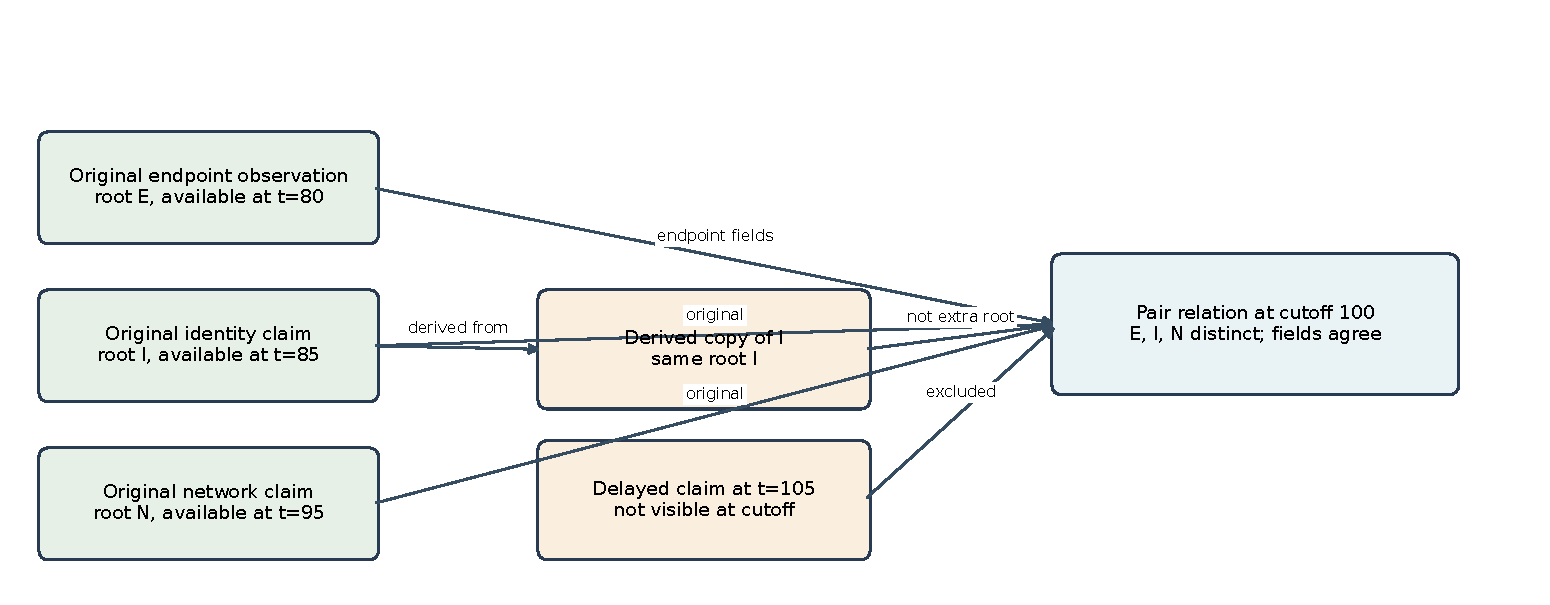
\includegraphics[width=.95\linewidth]{figures/evidence_provenance.pdf}\caption{Schematic point-in-time evidence record with illustrative minute values, not measured holdout observations. The original endpoint, identity, and network observations carry distinct roots E, I, and N. The derived identity copy retains root I, a contradictory observation cannot support the relationship, and an observation made at event minute 60 but available only at minute 105 is invisible at the minute-100 decision. Event time and evidence availability are different fields.}\label{fig:provenance}\end{figure}

\section{Correlation, verification, and prioritization architecture}
Figure~\ref{fig:arch} shows the deployed computational order and Figure~\ref{fig:pipeline} provides a data-flow summary with alert counts. The correlation routine first groups same-source alerts, process-tree references, and eligible lineage references with host/account guards and a component-size cap of 100. It returns a partition and candidate diagnostics. Verification then inspects each visible relationship-token bundle before any additional cross-fragment union. Finally the ranking routine orders the resulting groups for the analyst. The repository's earlier code labels this as C--P--V in places, but the frozen prediction call executes correlation, then verification, then scoring; we describe this actual execution order as C/V/P.

\begin{figure}[ht]
\centering
\includegraphics[width=\linewidth]{fig2}
\caption{Detailed evidence-token bundle processing within the verifier. Each claim bundle is checked for provenance roots, temporal availability, and claim consistency. Only bundles that pass all three checks—and satisfy component-context guards—may add a cross-fragment union.}
\label{fig:corrarch}
\end{figure}

Verification outcomes in the implementation are reason-coded. A mismatched event or causal field, late claim, shared root, derived-only family, excessive component size, or incompatible component host/account context prevents union. An absent process claim may be considered by the constrained fallback in Section~\ref{sec:method}; its extra check uses receiver-visible endpoint fields, not truth labels. Rejected and insufficient proposals leave the existing partition intact. This is a conservative decision procedure under its assumed root semantics, not a formal guarantee against adversarially coordinated false observations.
\begin{figure}[ht]\centering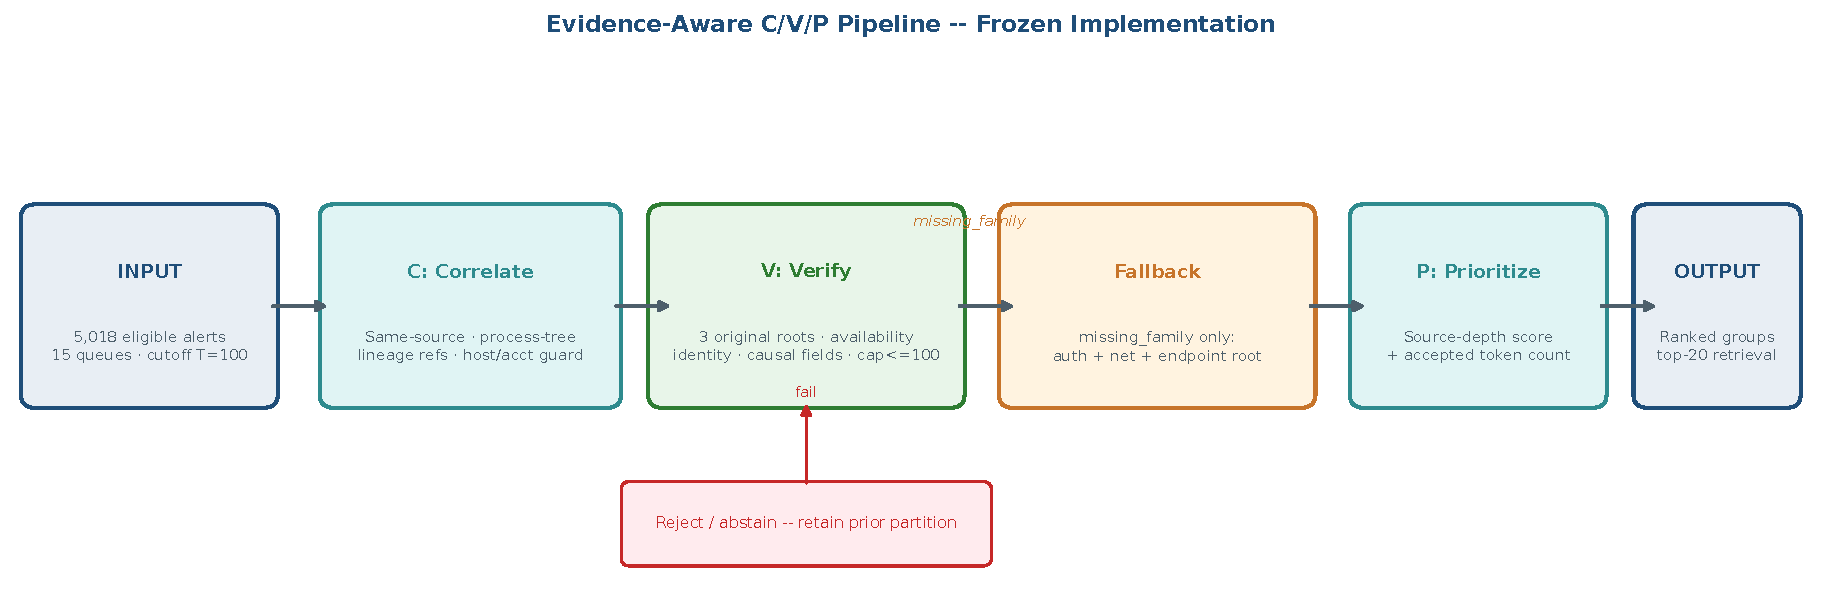
\includegraphics[width=\linewidth]{figures/pipeline_overview.pdf}\caption{Data-flow summary of the frozen C/V/P pipeline. The fallback branch is reachable only from the verifier for \texttt{missing\_family} rejections; all other failure modes retain the prior partition. Alert and queue counts are from the primary synthetic holdout (5,018 eligible alerts, 15 queues, cutoff $T=100$).}\label{fig:pipeline}\end{figure}

\section{Methodology}\label{sec:method}
\subsection{Visibility and initial fragments}
The receiver checks a contiguous evidence-ledger sequence, one availability record per alert, consistency between alert and ledger availability, and absence of private fields. It retains alerts and claims available by $T=100$, including only claims whose two endpoints are eligible. The initial correlator forms same-source and process-tree groups and tests available lineage references. Its host/account and component-cap guards operate on the current components; the standalone claim verifier does not retrospectively certify every initial within-source pair. Thus the zero false-pair observation is an evaluated property of this holdout, not a theorem of the verifier.

\subsection{Original independent attestation}
Claims are bundled by relationship token. The baseline's additional cross-fragment union requires exactly one original claim from each family $\{\mathrm{process},\mathrm{authentication},\mathrm{network}\}$, three distinct upstream roots, availability by $T$, identical endpoint/event identities, matching host/account, temporal compatibility, and matching process-parent, session, and flow identifiers. The event-time guard requires $t_b\geq t_a-3$ and $|t_b-t_a|\leq25$ minutes. A derived claim cannot replace an original family. Before union, the current components must share a host and an account and their combined size must not exceed 100.

The root and visibility checks are necessary conditions:
\begin{equation}\label{eq:gate}
\left|\{\rho(c):c\in B_r,\;c\text{ original}\}\right|=3,\qquad
\max_{c\in B_r}t_{\mathrm{available}}(c)\leq T.
\end{equation}
Equation~\ref{eq:gate} does not alone imply acceptance: all identity, context, time, and component checks must also pass. The verifier logs a failed reason and leaves the partition unchanged. Each token's attestation is checked against original alert fields; newly joined components do not create synthetic support for a subsequent token. Union operations themselves are transitive, so the final group can contain alerts joined through multiple separately checked tokens.

\subsection{Constrained endpoint fallback}
The candidate retries only rejected tokens with reason \texttt{missing\_family}. It requires exactly two original claims, one authentication and one network-flow claim, with distinct roots and availability by 100. The two endpoint alerts must themselves be original, from different source and observation identifiers, with a common endpoint-origin root that differs from both claim roots. Their host, account, event timing, process-parent, authentication-session, and flow identifiers must agree. Every claim in the bundle must agree with endpoint fields; component host/account overlap and cap checks are reapplied. The endpoint observation serves as the missing process-family witness. Other rejection reasons are not relaxed. Figure~\ref{fig:verify} traces these gates.
\begin{figure}[ht]\centering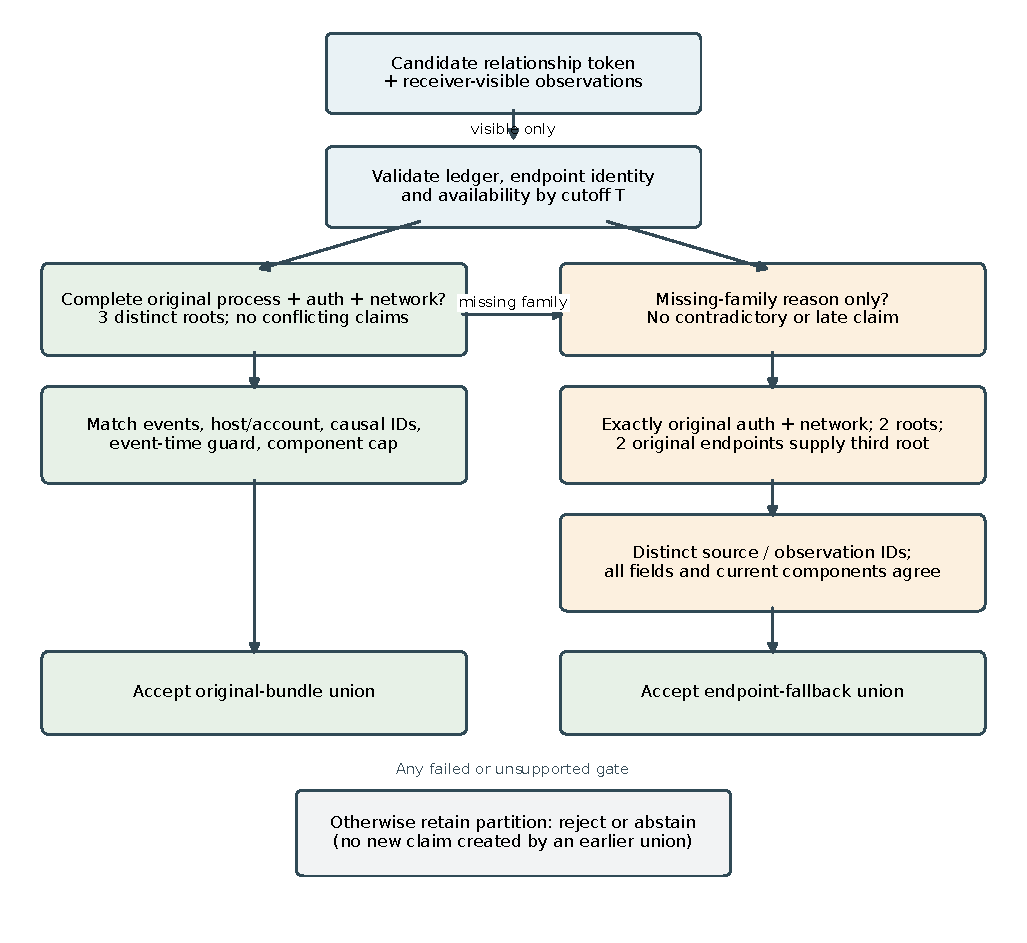
\includegraphics[width=\linewidth]{figures/verification_methodology.pdf}\caption{Relationship-token verification. A complete original process/authentication/network bundle can pass the baseline verifier. Only a missing-process-family rejection enters the endpoint fallback, which requires two original claim roots plus a third endpoint root. Identity, field, temporal, component-context, and size checks remain mandatory. Failed or unsupported tokens do not change the existing groups.}\label{fig:verify}\end{figure}

\subsection{Grouping and scoring}
Both arms rank by source depth: $1.2$ times maximum severity, $0.7$ times maximum asset criticality, $0.55$ times distinct event types, and $0.7$ times the number of distinct sources capped at 10. The frozen baseline adds one point per accepted token whose left endpoint is in the group. The candidate uses the same bonus coefficient of one and includes fallback unions. Groups are sorted by descending score and then first alert identifier. A group never becomes recoverable merely because its rank changes; Figure~\ref{fig:groups} separates grouping from top-20 retrieval.
\begin{figure}[ht]\centering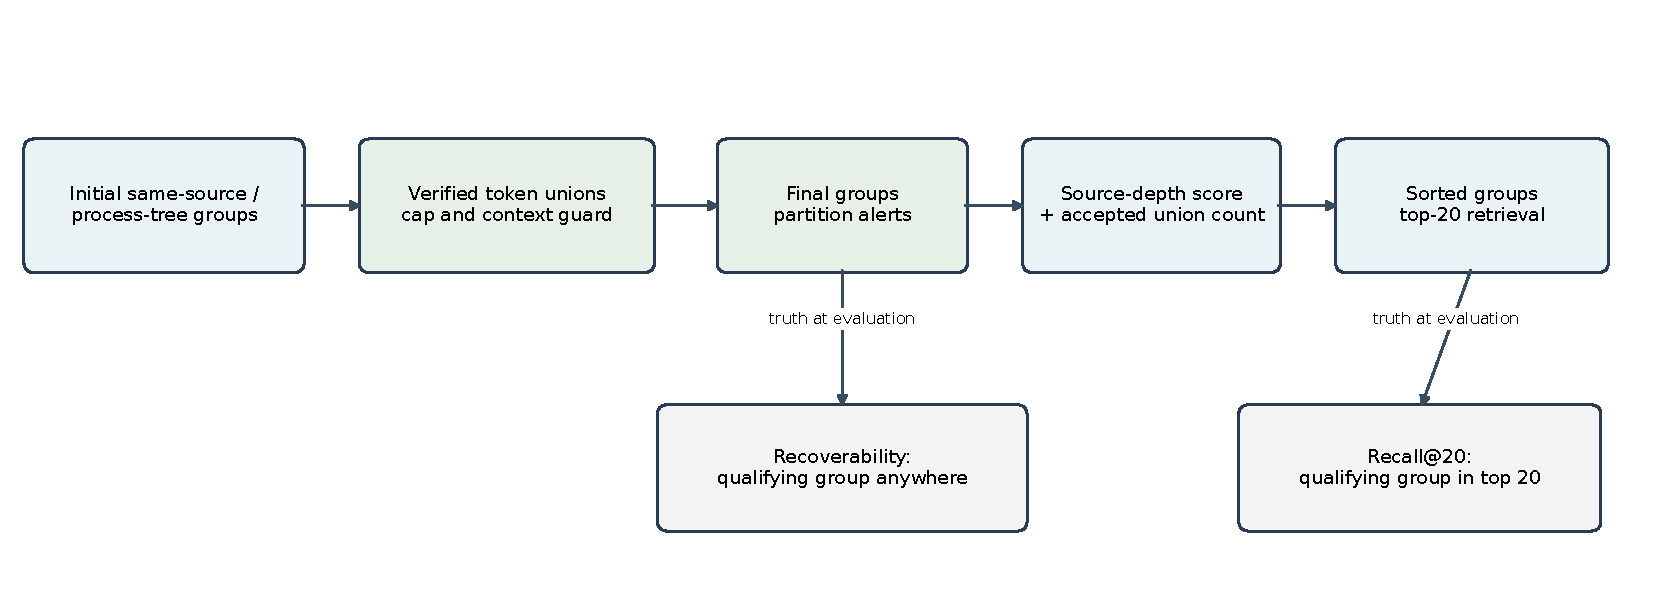
\includegraphics[width=\linewidth]{figures/reconstruction_prioritization.pdf}\caption{Initial fragments and accepted evidence-token unions form the final partition. Scoring orders these fixed groups. The evaluator separately checks whether an expert incident has a sufficiently complete and pure group anywhere (recoverability) and whether one appears within the first 20 (Recall@20); ranking cannot create a missing group.}\label{fig:groups}\end{figure}

\section{Experimental design}
The primary comparison uses a controlled synthetic evidence generator with process, authentication, and network-flow claims, original/derived observations, missing and contradictory fields, and recorded availability minutes. Eight training queues and ten development queues (200 expert top-20 opportunities) supported method development. The frozen development candidate obtained 169/200 Recall@20, 177/200 recoverability, and 73/100 P@10, with no false grouped pairs or mixed groups. It missed the predeclared 170/200 development gate by one incident. A documented subsequent decision permitted evaluation of the unchanged candidate on a new holdout; this was a protocol adjustment, not a passed development gate.

\begin{figure}[ht]
\centering
\includegraphics[width=\linewidth]{fig3}
\caption{Experimental protocol overview: controlled training, development with the missed gate condition, documented authorization, and frozen holdout evaluation. Source/prediction hashes were SHA-256 sealed before private-truth access. No post-result holdout tuning occurred.}
\label{fig:expoverview}
\end{figure}

The holdout used seed 31103, template variant 2, and 15 queues, with 5,018 eligible alerts and 300 expert top-20 opportunities. Baseline and candidate predicted the same alert sets. Source/configuration hashes were frozen; prediction and decision files were SHA-256 sealed before the unchanged evaluator accessed private truth. Each arm was evaluated once. The holdout is within the synthetic generator family and uses a distinct template variant; it is not an operational dataset. Figures~\ref{fig:protocol} and~\ref{fig:devtraj} illustrate the experimental separation and development trajectory.
\begin{figure}[ht]\centering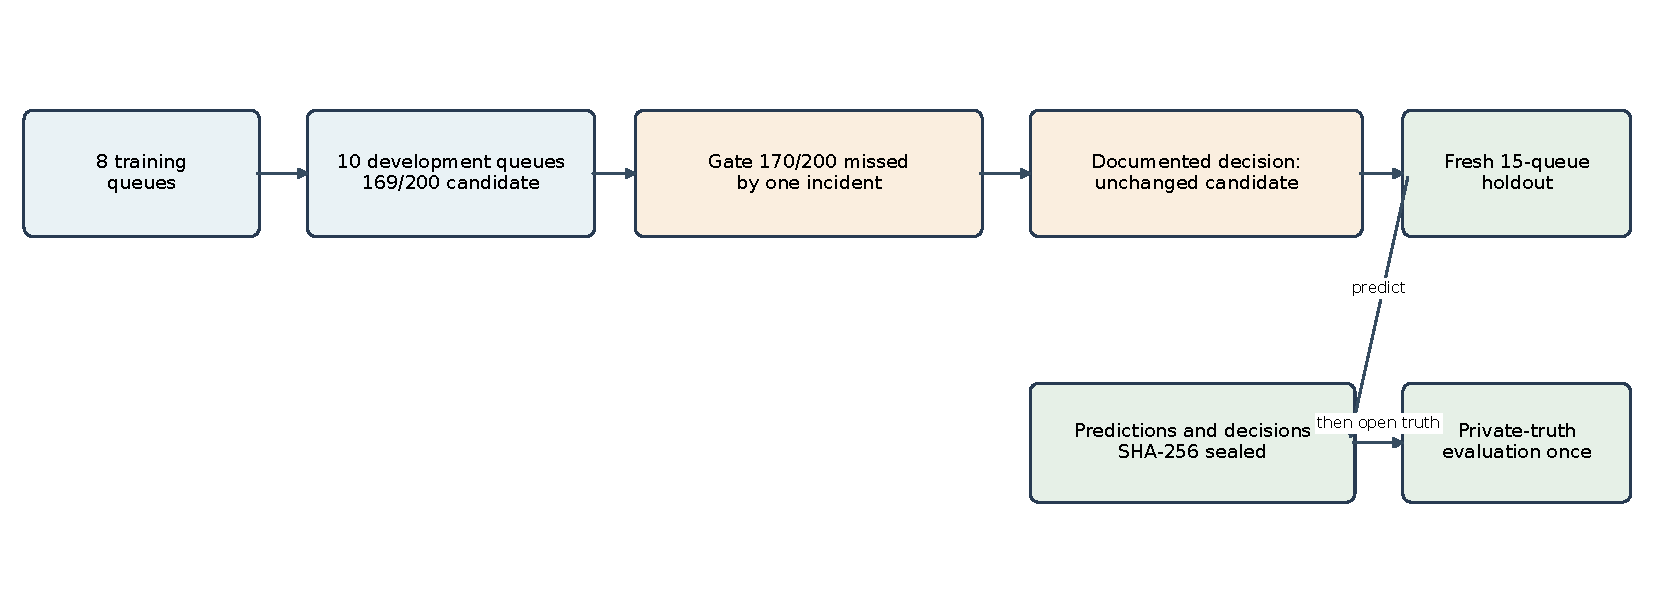
\includegraphics[width=\linewidth]{figures/experimental_protocol.pdf}\caption{Experimental order: training and development, the missed 170/200 development gate, the documented authorization to test the unchanged candidate, a fresh synthetic holdout, SHA-256 sealing, and one subsequent private-truth evaluation. No post-result holdout tuning is represented.}\label{fig:protocol}\end{figure}
\begin{figure}[ht]\centering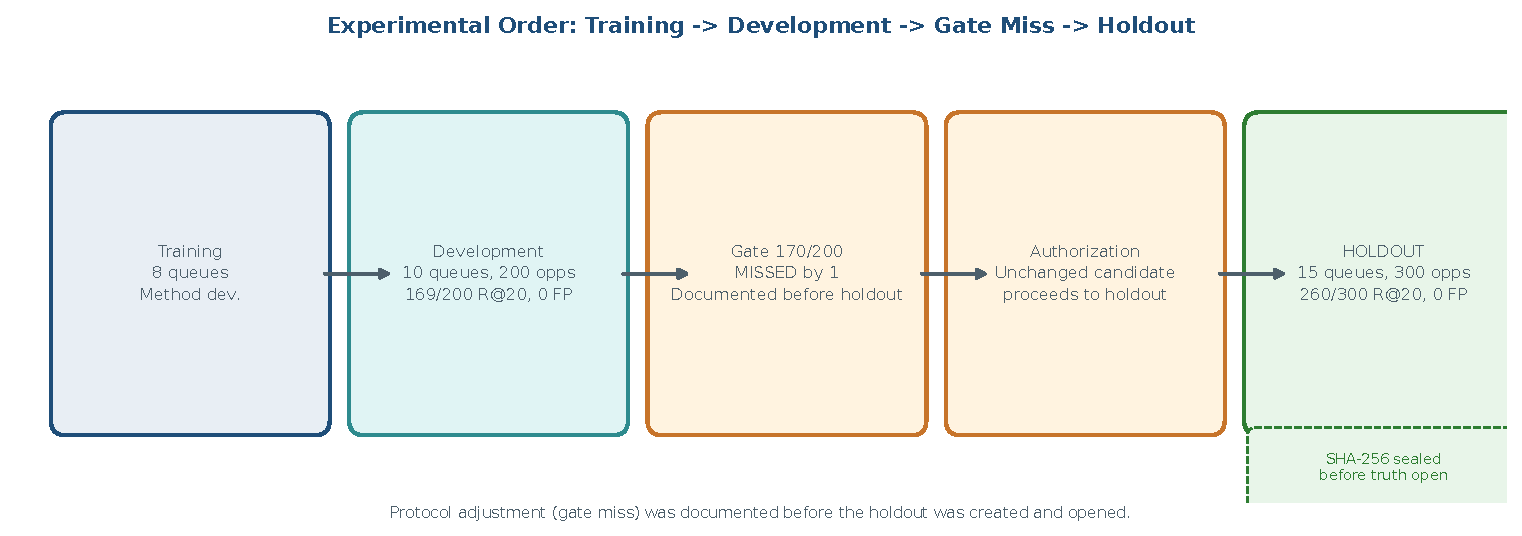
\includegraphics[width=\linewidth]{figures/dev_trajectory.pdf}\caption{Annotated development trajectory from training through holdout. The gate miss and authorization decision are shown explicitly; both occurred before the holdout population was created or any truth label was accessed.}\label{fig:devtraj}\end{figure}

\begin{table}[ht]\centering\small\caption{Distinct research populations. Separate development cohorts in later studies cannot be pooled with the primary holdout.}\label{tab:cohorts}\begin{tabularx}{\linewidth}{@{}p{32mm}p{27mm}Y@{}}\toprule Population & Size & Role and boundary\\\midrule Controlled training & 8 queues & Generator-family method development; private holdout not involved\\ Controlled development & 10 queues; 200 top-20 opportunities & Candidate selection and one-incident gate miss\\ Frozen holdout & 15 queues; 5,018 eligible alerts; 300 top-20 opportunities & Paired baseline/candidate evaluation after prediction seal\\ Later studies & Separate development cohorts, generally 15 queues each & Diagnostic and ranking investigations; no fresh promoted holdout\\ GUIDE inspection & 4,147,992 evidence rows & Schema/readiness audit; no model predictions\\\bottomrule\end{tabularx}\end{table}

\section{Evaluation metrics}
The evaluator has 25 expert-priority incidents per queue and takes ranks 1--20 as the target set. Let $n_i$ be the number of eligible alerts for incident $i$, $h_{iG}$ the number of those in predicted group $G$, and $|G|$ its size. A group qualifies for $i$ if
\begin{equation}\label{eq:qualify}Q(i,G)=\mathbf{1}\left[\frac{h_{iG}}{n_i}\geq0.8\;\land\;\frac{h_{iG}}{|G|}\geq0.8\right].\end{equation}
The denominator $n_i$ concerns eligible alerts, not all generated alerts. Every expert incident must have at least one eligible alert. If any group qualifies, $i$ is recoverable; if any qualifying group has rank at most 20, it is recalled. For $N$ queues, the implementation micro-aggregates counts:
\begin{equation}\label{eq:recall}
R@20=\frac{\sum_q\sum_{i\in I_q^{20}}\mathbf1[\exists G:\,Q(i,G)=1\land \operatorname{rank}(G)\leq20]}{20N},\quad
\operatorname{Recov}=\frac{\sum_q\sum_{i\in I_q^{20}}\mathbf1[\exists G:\,Q(i,G)=1]}{20N}.
\end{equation}
For P@10 the evaluator scans the first 20 groups, credits at most one previously uncredited qualifying incident per group (lowest expert rank if several qualify), and counts a credit only when the group is within positions 1--10 and the incident's expert rank is at most 10. The aggregate denominator is $10N$. This assignment rule is more specific than ordinary binary relevance precision.

For each group, the evaluator counts true within-group pairs $\sum_i\binom{h_{iG}}2$ and false within-group pairs $\binom{|G|}2-\sum_i\binom{h_{iG}}2$. Grouped-pair precision is total true divided by total true plus false pairs across queues; its implementation defines precision as one when no pairs exist. False grouped pairs is the summed false count. A mixed group is any predicted group containing more than one truth incident, even if it passes the 80\% purity threshold. These safety measures include all groups, not just the top 20. Candidate-edge precision is not recoverable from the prediction artifact and is not reported.

\section{Results}
\subsection{Primary frozen synthetic holdout}
Table~\ref{tab:primary} and Figure~\ref{fig:primary} show the paired comparison on exactly the same 15 queues. The candidate recovered 18 additional expert top-20 incidents and recalled 10 additional incidents in the first 20 groups. P@10 rose by six credited positions. These are absolute differences of 6.00, 3.33, and 4.00 percentage points, respectively; no statistical significance claim is made.
\begin{table}[ht]\centering\small\caption{Frozen paired holdout results. Fractions use evaluator opportunity denominators. Differences are candidate minus baseline; percentage differences are percentage points.}\label{tab:primary}\begin{tabularx}{\linewidth}{@{}Yrrr@{}}\toprule Metric & Frozen baseline & Endpoint fallback & Difference\\\midrule Incident Recall@20 & 250/300 (83.33\%) & 260/300 (86.67\%) & +10 (+3.33 pp)\\ Group recoverability & 263/300 (87.67\%) & 281/300 (93.67\%) & +18 (+6.00 pp)\\ P@10 & 107/150 (71.33\%) & 113/150 (75.33\%) & +6 (+4.00 pp)\\ Grouped-pair precision & 19,459/19,459 (100\%) & 20,117/20,117 (100\%) & 0 pp\\ False grouped pairs & 0 & 0 & 0\\ Mixed groups & 0 & 0 & 0\\\bottomrule\end{tabularx}\end{table}
\begin{figure}[ht]\centering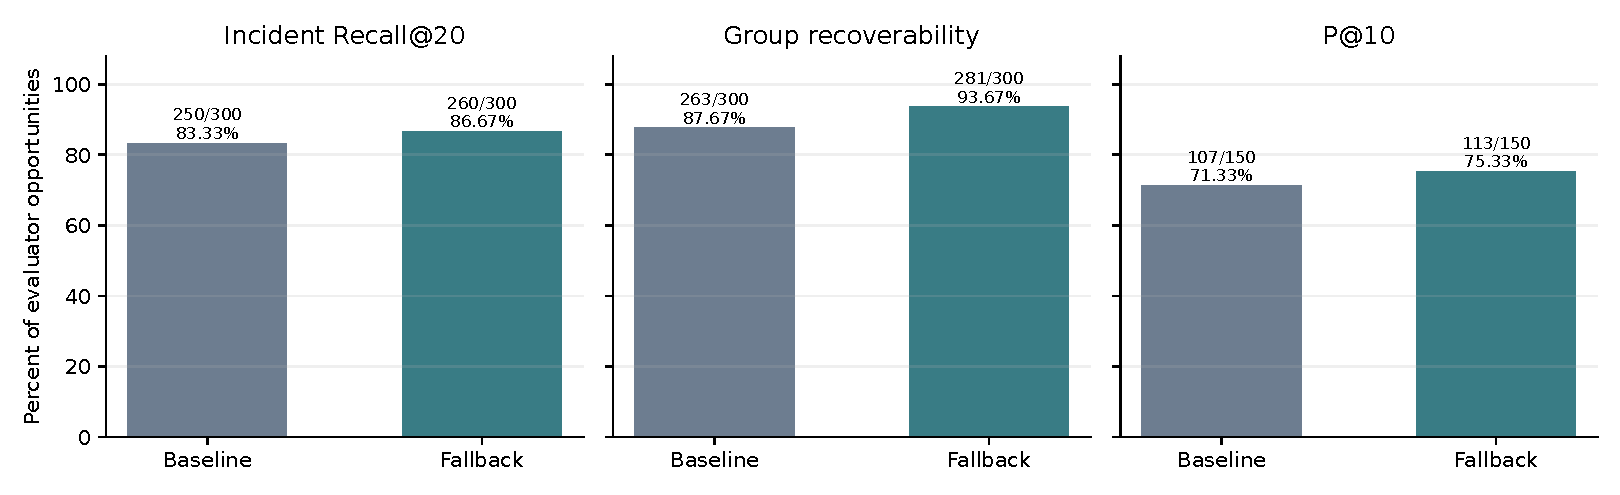
\includegraphics[width=\linewidth]{figures/phase33_results.pdf}\caption{Frozen synthetic holdout metrics generated directly from the verified holdout summary, with exact counts and evaluator denominators. Axes run from zero to allow direct comparison; the three panels represent different evaluation opportunities and must not be added together.}\label{fig:primary}\end{figure}

The simulator-truth audit classified all 28 newly accepted fallback unions and all 711 total candidate accepted unions as genuine. It recorded 150 false relationship-token rejections and 35 genuine-token abstentions. These token counts refer to a different evaluation unit than pair precision. Figure~\ref{fig:safety} displays the all-group safety results; all 15 queues had zero false pairs and zero mixed groups in both arms. Queue-level Recall@20 nevertheless fell by one incident in two queues, and P@10 fell in two queues. Aggregate gains therefore do not imply uniform queue gains.
\begin{figure}[ht]\centering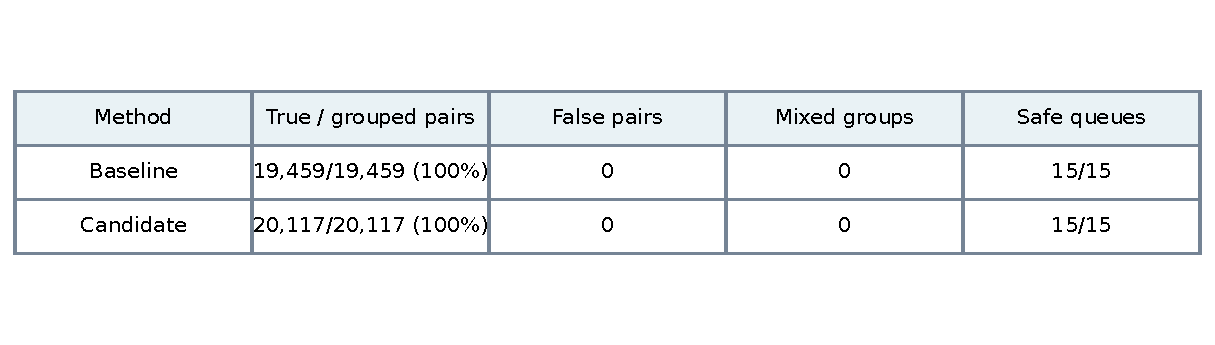
\includegraphics[width=.9\linewidth]{figures/safety_results.pdf}\caption{Grouped-pair and mixed-group outcomes on the 15-queue controlled holdout. Pair precision uses all within-group pairs; the count of safe queues is based on zero false grouped pairs and zero mixed groups in each queue. Zero observed errors under simulator truth is not a bound on real-world error rates.}\label{fig:safety}\end{figure}

\subsection{Development-only and historical evidence}
Table~\ref{tab:development} summarizes separate ranking and evidence studies. Later development scores are not substituted for the frozen holdout or construed as a performance trajectory. The earlier historical synthetic holdout had 407/600 Recall@20 and 451/600 recoverability on another population; its scores are not directly comparable. An unsafe richer-claim development configuration produced 2,580 false pairs and 22 mixed groups, whereas independent-claim verification on that development cohort preserved zero false pairs and recovered 166/200 incidents.
\begin{table}[ht]\centering\small\caption{Later investigations on distinct development-only cohorts. B and C are matched within each row; they are not comparable across rows as successive improvements.}\label{tab:development}\begin{tabularx}{\linewidth}{@{}p{29mm}Yrrr@{}}\toprule Study & Question & Baseline R@20 & Candidate R@20 & Candidate recoverability\\\midrule Ranking feature study & Post-group score & 264/300 & 267/300 & 277/300\\ Near-boundary rank study & Reorder below first ten & 258/300 & 258/300 & 273/300\\ Evidence-aware rank study & Visible evidence features & 265/300 & 262/300 & 277/300\\ Evidence availability & Frozen condition, stress tests & 257/300 & --- & 267/300\\ Hard-negative rank study & Pairwise trained reordering & 263/300 & 262/300 & 279/300\\\bottomrule\end{tabularx}\end{table}

\section{Discussion}
The endpoint fallback increases recoverability because it permits a missing process claim to be replaced by original endpoint context while retaining original identity and network corroboration. The difference between +18 recoverable and +10 recalled incidents illustrates that reconstruction and ranking are separate bottlenecks. A high grouped-pair precision does not guarantee useful retrieval, nor does it validate source independence outside the simulator.

The verifier refuses a derived copy as a new root and filters claims by evidence availability rather than event time. Stress studies on separate development populations showed lower recovery with delayed, absent, corrupted, or contradictory evidence. A purported fourth independent source was unavailable; no substitute observations were invented. Later ranking attempts kept grouping fixed and failed to establish a consistent top-20 gain. In particular, a pairwise-trained ranker reduced matched development recall from 263/300 to 262/300 even while preserving the partition. Its training objective was not the evaluator's top-20 incident objective.

This design deliberately trades some recoverability for a narrow acceptance rule. Thirty-five genuine relationship tokens were abstained on in the primary holdout, while no false grouped pairs were observed. Whether this tradeoff is appropriate for a SOC depends on the cost of missed incidents, the quality of independent telemetry, and review workflow; those operational quantities were not measured.

\section{Threats to validity}
The principal threat is synthetic-to-operational transfer. The generator defines incident truth, root identifiers, causal fields, and challenging counterexamples. Distinct simulated roots do not prove that real identity-provider, network, and endpoint controllers are independent or resistant to coordinated corruption. The holdout shares a generator family with development, has 15 queues, and cannot support a broad operational error-rate estimate.

The candidate missed its original development Recall@20 gate by one incident. The later decision to proceed unchanged was recorded before creating and opening the fresh holdout, but the adjustment weakens the strength of a strict preregistered selection claim. Metric conclusions depend on the 80\% completeness/purity qualification rule and the simulator's expert-priority labels. Pair precision counts all within-group pairs and can be dominated by large correct groups. The baseline's initial grouping is not subject to the same three-root gate as extra verified unions. Later cohorts differ in seeds and challenge compositions; comparing their raw percentages as though paired would be invalid.

No authorized external SOC ground truth and no real point-in-time provenance ledger were available. We therefore have no estimate of real false unions, analyst utility, workload, latency distribution, or cost of abstention.

\section{External evaluation readiness}
The local Microsoft GUIDE inspection found 4,147,992 evidence rows, 637,320 composite alert keys, 303,220 composite incident keys, and 9,980 ranking rows. It also found 70,702 composite alert keys assigned to conflicting incidents. GUIDE documentation describes timestamp perturbation; its alert-creation timestamp is not the receiver's evidence-availability time \citep{guide2024}. The available export lacked original source-observation identifiers, upstream trust roots, derivation chains, and independently supported process/authentication/network relationship bundles. Queue scope, rank direction, and complete analyst-priority semantics remained unresolved. The existing field policy authorized zero real model-visible fields.

\begin{table}[ht]\centering\small\caption{External data-readiness audit. Missing fields prevent evaluation of the frozen rule without changing its inputs or admitting future/private information.}\label{tab:readiness}\begin{tabularx}{\linewidth}{@{}p{35mm}Y Y@{}}\toprule Requirement & Observed condition & Consequence\\\midrule Original observation IDs, roots, derivation & Not available in local GUIDE fields & Three-root independence cannot be checked\\ Point-in-time availability & Creation timestamp noised; ingestion history absent & Cutoff filtering cannot be reproduced\\ Causal process/auth/network claims & No verified bundles for frozen rule & Frozen verifier cannot operate on equivalent input\\ Alert and incident truth & 70,702 composite alert keys have conflicting assignments & Incident qualification requires resolution\\ Queue and priority semantics & 9,980 ranking rows; scope/direction unresolved & Top-20 denominator/meaning uncertain\\ Approved visible fields & None approved & No authorized real input to the model\\\bottomrule\end{tabularx}\end{table}

Consequently evaluation stopped before any real-data prediction. No real-world Recall@20, pair precision, or deployment metric exists for this study. This is a data-readiness failure, not evidence that the method succeeded or failed on real SOC data.

\section{Limitations and future work}
A credible external study requires a separately authorized SOC cohort with original observation identity, verifiable upstream provenance and derivation, evidence ingestion times, independently adjudicated incident membership, queue scope, analyst rank direction, and a declared list of visible fields. A new protocol should freeze the method and exclusions before labels are opened, retain abstention and false-merge outcomes, compare compatible baselines, and evaluate sensitivity to shared-controller failure and coordinated false evidence. Repeated tuning on the existing synthetic cohorts would not resolve the external-validity gap.

\section{Conclusion}
We examined a correlation and prioritization pipeline whose additional cross-fragment unions require original, timely, independently rooted evidence and field consistency. A constrained endpoint fallback improved synthetic holdout Recall@20 from 250/300 to 260/300 and recoverability from 263/300 to 281/300, with zero observed false grouped pairs or mixed groups in both arms. The candidate's missed development gate and documented holdout-protocol adjustment qualify this result. External validation remains unperformed because the available real-data fields cannot support the frozen evidence and evaluation requirements. The next scientific test is a predeclared evaluation on authorized, point-in-time, independently sourced SOC evidence.

\bibliographystyle{unsrtnat}\bibliography{references}
\appendix\section{Verification and grouping procedure}
For each queue, the frozen implementation filters alerts and claims by availability, forms initial source/process/lineage groups, then iterates token bundles in sorted order for complete three-family attestations. Rejected tokens whose sole reason is missing family enter the endpoint fallback. Every accepted token unites its current endpoint components only after size and context checks. A successful union never produces a new original claim or root. The baseline and candidate finally score each group and sort by descending score and first alert identifier. The executable specification is \texttt{experiments/PHASE31\_CONTROLLED\_SOC\_EVIDENCE/model.py}, \texttt{experiments/PHASE32\_SAFE\_EVIDENCE\_RECOVERY/model.py}, and the frozen earlier correlator.
\section{Queue-level outcome and artifact trail}
The editable per-queue counts and figure-generation data are in \texttt{figure\_data/holdout\_queue\_metrics.csv}, \texttt{figure\_data/holdout\_metrics.csv}, and \texttt{figure\_data/holdout\_safety.csv}. The original sealed predictions and private-truth evaluation remain in the research repository. No historical experiment output is regenerated by the paper build.

\end{document}
